\documentclass[]{article}

% Packages
\usepackage{amsmath} % math stuff
%\usepackage[dvipsnames]{xcolor}  % for coloring
\usepackage{tensor}  % tensors, but also for stuff like superscript on the left
\usepackage{enumitem} % for enumerating alphabetically
\usepackage{tabto}		% for tabbing to a certain length
\usepackage{scrextend} % for local margins
\usepackage{titling}	% for subtitle custom command
\usepackage[svgnames, table]{xcolor} % avoid the option clash for hyperref command  + TABLE REP
\usepackage[colorlinks=true, linkcolor=Blue, urlcolor=Blue]{hyperref} % for hyperref command 
\usepackage{pgfplots} % plots
\usepackage{physics}	%derivative (\dv)+ and more
\usepackage{outlines} % convienent itemizing
%%\usepackage{multirow} % multiple rows for tables
\usepackage{bm}	% bold math
\usepackage{systeme}	% for systems of equations

%for flowchart:
\usepackage{amsmath}
\usepackage{amssymb}
\usepackage{graphicx}
\usepackage{siunitx}
\usepackage{tikz}
\usetikzlibrary{patterns}
\usepackage{caption}
\usetikzlibrary{arrows}
\usepackage{color}
\usepackage{pgfplots}
\usepackage{listings}
\usepackage[utf8]{inputenc}
\usetikzlibrary{shapes.geometric}
\usepackage{tikz-cd}
\usetikzlibrary{positioning}
\tikzset{
	shift left/.style ={commutative diagrams/shift left={#1}},
	shift right/.style={commutative diagrams/shift right={#1}}
}


%tables for list representation
\usepackage{arydshln, collcell}
\newcolumntype{C}{>{\collectcell\mathsf}c<{\endcollectcell}}

% Python code
\definecolor{codegreen}{rgb}{0,0.6,0}
\definecolor{codegray}{rgb}{0.5,0.5,0.5}
\definecolor{codepurple}{rgb}{0.58,0,0.82}
\definecolor{codeblue}{rgb}{0.08,0.1,0.87}
\lstdefinestyle{pystyle}{
	language=Python,   
	commentstyle=\color{codegreen},
	keywordstyle=\color{codeblue},
	numberstyle=\tiny\color{codegray},
	stringstyle=\color{codepurple},
	basicstyle=\ttfamily\footnotesize,
	breakatwhitespace=false,         
	breaklines=true,                 
	captionpos=b,                    
	keepspaces=true,                 
	numbers=left,                    
	numbersep=5pt,                  
	showspaces=false,                
	showstringspaces=false,
	showtabs=false,                  
	tabsize=2
}
\lstset{style=pystyle}

%Repeat command
\usepackage{expl3}
\ExplSyntaxOn
\cs_new_eq:NN \Repeat \prg_replicate:nn
\ExplSyntaxOff

% Algorithms
\usepackage{algorithm}
\usepackage{algorithmicx}
\usepackage[noend]{algpseudocode}
\newcommand{\Get}{\State \textbf{get}~}
\newcommand{\Set}{\State \textbf{set}~}
\newcommand{\Print}{\State \textbf{print}~}
\newcommand{\Getx}[1]{\Statex \algindent{#1} \textbf{get}~}		% x denotes non-numbered lines
\newcommand{\Setx}[1]{\Statex \algindent{#1} \textbf{set}~}	% enter the number of lines to indent
\newcommand{\Printx}[1]{\Statex \algindent{#1} \textbf{print}~}
\newcommand{\Stop}{\State \textbf{stop}~}
\newcommand{\algindent}[1]{\Repeat{#1}{\hskip\algorithmicindent}}
\algdef{SE}[DOWHILE]{Do}{doWhile}{\algorithmicdo}[1]{\algorithmicwhile\ (#1)}

% plots
\usepackage{pgfplots}
\usepgfplotslibrary{fillbetween}
\pgfplotsset{compat=1.15} 

% stop indentation
\setlength{\parindent}{0pt}

% custom subtitle command
\newcommand{\subtitle}[1]{
	\posttitle{
		\par\end{center}
	\begin{center}\large#1\end{center}
	\vskip0.5em}
}


% Fixes weird backwards quote thing
\usepackage [english]{babel}
\usepackage [autostyle, english = american]{csquotes}
\MakeOuterQuote{"}

% fix upside down exclaimation points for less thans or greater thans
\usepackage[T1]{fontenc}


% Title
\title{PHY 325 Notes}
\subtitle{Computational Physics}
\author{Jaeden Bardati}
\date{\textit{Last modified \today}}

%\setcounter{section}{-1}	% 0-indexes the section

\begin{document}

\maketitle
\bigbreak

\section{Numerical Evaluation of Derivatives}\bigbreak\bigbreak


Let $y = f(x)$, then the \textbf{derivative} is defined as

\begin{equation}\label{eq:limit-definition-of-derivative}
	\dv{f}{x} \equiv \mathop {\lim }\limits_{h \to 0} \frac{{f\left( {x + h } \right) - f\left( x \right)}}{h }
\end{equation}\bigbreak

Now consider $y = f(x_1, ..., x_n)$, then the \textbf{partial derivative} is defined as

\begin{equation}\label{eq:limit-definition-of-partial-derivative}
	\pdv{f}{{x_i}} \equiv \mathop {\lim }\limits_{h \to 0} \frac{{f\left( {x_1, ..., x_{i}+h, ..., x_n} \right) - f\left(x_1, ..., x_n \right)}}{h }
\end{equation}\bigbreak

We can numerically compute derivatives in three main ways: forwards, backwards and with an average of the two.\\

The \textbf{forward} derivative is defined as

\begin{equation}\label{eq:forward-derivative}
	\dv{f}{x} \approx \frac{{f\left( {x + h } \right) - f\left( x \right)}}{h}
\end{equation}\bigbreak

The \textbf{backward} derivative is defined as

\begin{equation}\label{eq:backward-derivative}
	\dv{f}{x} \approx \frac{{f\left( {x - h } \right) + f\left( x \right)}}{h}
\end{equation}\bigbreak

The \textbf{central} derivative is defined as

\begin{equation}\label{eq:central-derivative}
	\dv{f}{x} \approx \frac{{f\left( {x + h } \right) - f\left( x - h \right)}}{2h}
\end{equation}\bigbreak

The smaller $n$ is, the more accurate this approximation is.\\

Note that, while the forward and backward derivatives take the same amount of time to compute, the central derivative has twice the number of calculations to do and so will take longer to run.\\ 

Furthermore, the central derivative can have divergent behaviour. To illustrate this, we can take the central derivative at the point (0, 0) on the absolute value function (see figure \ref{fig:absolute-value}). Notice that the value of the derivative is 0 here, which could lead to undesired effects in the simulations of such systems.\\

\begin{figure}[th!]
	\centering
	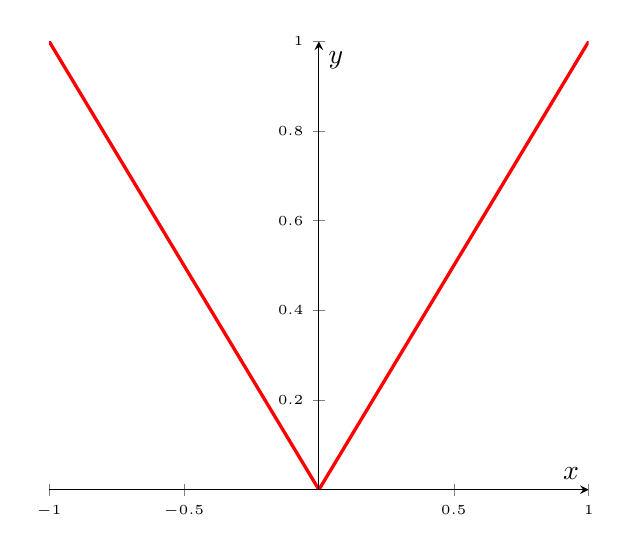
\begin{tikzpicture}
		\begin{axis}[
			axis on top,
			legend pos=outer north east,
			axis lines = center,
			xticklabel style = {font=\tiny},
			yticklabel style = {font=\tiny},
			xlabel = $x$,
			ylabel = $y$,
			legend style={cells={align=left}},
			legend cell align={left},
			]
			\addplot[very thick,red,samples=161,domain=-1:1,name path=f] {abs(x)};
		\end{axis}
	\end{tikzpicture}
	\caption{Absolute value function} \label{fig:absolute-value}
	\bigbreak
\end{figure}

\section{Error in Derivative Calculation}\bigbreak\bigbreak

When implementing a numerical derivative calculation, we would like to use a small value of $h$. But how small? One might think that we should try to make $h$ as small as it can be. Of course, zero will not work since it would result in an error due to division by 0 (see equations \ref{eq:forward-derivative}, \ref{eq:backward-derivative}, and \ref{eq:central-derivative}). \\

If we plot $h$ by the error in the derivative, we will find that the derivative is inaccurate at both high and low values for $h$. There is a "sweet spot" in the middle (roughly around $10^{-8}$) that minimizes the error. The error at low values of $h$ is called \textbf{round-off error} and at high values of $h$ is called \textbf{truncation error}.\\

\subsection{Round-off Error}\bigbreak

To understand this error, we must first ask: How are numbers represented by a computer? Specifically, we are interested in floats. The form is:

\begin{equation}
	s \times M \times B^{e - E}
\end{equation}

where $s$ is the sign (0 if number is positive, 1 if negative), $M$ is the Mantissa, $B$ is the base, $E$ is the bias, and $e$ is the exponent. \\

This form is similar to scientific notation in principle. Namely, it is much more space-efficient to write $1.2 \times 10^{-8}$ rather than 0.000000012. Note that here, 1.2 is the Mantissa, 10 is the base, the sign is 0, and $e-E = -8$.\\

For example, we will look at how 10.75 is stored. In binary, $(10)_{10} = (1010)_{2}$ and $(0.75)_{10} = (11)_2$, where the subscript indicates the base). So, 

\[(10.75)_{10} =  (1010.11)_{2} = (1.01011)_{2} \times 2^3\]\bigbreak

The bias term $E$ is highly dependent on the particular machine you use. However, for a typical 32-bit computer, it is common to have a bias of $E = 2^{n-1} + 1$ with $n=8$. This gives that $E=129$. The base is, of course, $B=2$. \\

Calculating $e$ now, we know

\[e - E = 3 \implies e = 3 + E = 3 + 129 = 132\]\bigbreak

In binary, $(132)_{10} = (10000100)_2$.\\

Therefore, we would store the float value of 10.75 as

\begin{table}[h]\centering
	\begin{tabular}{|c|c|c|}
		\hline
		0 & 10000100 & 10101100000...000\\\hline
		\multicolumn{1}{c}{$s$} & \multicolumn{1}{c}{$e - E$} & \multicolumn{1}{c}{$M$ (23-bits)}
	\end{tabular}
\end{table}

In a 32-bit system, 1 bit is used to store the sign $s$, 8 bits for the exponent $e-E$, and 23 bits for the mantissa $M$. In a 64-bit system (double precision), 1 bit is used to store the sign $s$, 11 bits for the exponent $e-E$, and 52 bits for the mantissa $M$. \\

Since the mantissa is only a certain size, once a decimal value becomes lower than what can be stored in the mantissa, the value is lost. This is round-off error. The machine accuracy for a 32-bit system is around $10^{-8}$ and for a 64-bit system is $10^{-16}$.\\

It is important when analyzing numerical systems to pick normalized units (close to unity). That is to say, choose units such that the numbers that are being used do not have this round-off error effect. \\

\subsection{Truncation Error}\bigbreak

Truncation error has to do with the sort of "rate of error decreasing with respect to h." Namely, if we Taylor expand $f(x+h)$, we obtain

\[f(x+h) = f(x) + hf'(x) + \frac{1}{2}h^2f''(x) + \frac{1}{6}h^3f'''(x) + ...\] 

So, the calculation we use for the forward derivative (equation \ref{eq:forward-derivative}) is

\begin{align*}
	\frac{f(x+h) - f(x)}{h} &= f'(x) + \frac{1}{2}hf''(x) + \frac{1}{6}h^2f'''(x) + ...\\
	\implies \frac{f(x+h) - f(x)}{h} &\approx f'(x) + O(h)
\end{align*}

We can see that the forward derivative is only accurate to the first order of $h$. This is why there is an increase in error when $h$ is large. It is called \textbf{truncation error} since we truncate the infinite series when approximating.

\section{Example: Projectile Motion}\bigbreak\bigbreak

Consider a baseball thrown with air resistance. The equations of motion are

\begin{align}
	\dv{\vec{v}}{t} &= \frac{1}{m}\vec{F}_{\text{air}}(v) - g\hat{y}\\
	\dv{\vec{r}}{t} &= \vec{v}
\end{align}

where $\vec{v}$ is the velocity, $t$ is the time elapsed, $m$ is the mass of the baseball, $g$ is the gravitational acceleration, $\hat{y}$ is the upward direction, and $\vec{r}$ is the position vector. Note that the force of air friction here is 

\begin{equation}
	\vec{F}_{\text{air}}(v) = -\frac{1}{2} C_d \rho A |\vec{v}|\vec{v}
\end{equation}

where $C_d$ is the coefficient of air friction, $\rho$ is the density of air, and $A$ the area of the baseball (perpendicular to its direction of travel).

\subsection{Euler Method}\bigbreak

The Euler method is a numerical procedure for solve initial value problems of ordinary differential equations. Namely, if we have the form

\begin{align*}
	\dv{\vec{v}}{t} &= \vec{a}(\vec{r}, \vec{v})\\
	\dv{\vec{r}}{t} &= \vec{v}
\end{align*}

where $\vec{a}(\vec{r}, \vec{v})$ is the acceleration vector as a function of the position and velocity vectors.\\

Using the forward derivative where $\tau = h$ represents an increment in the time, then

\begin{align*}
	\frac{\vec{v}(t + \tau)-\vec{v}(t)}{\tau} &= \vec{a}(\vec{r}, \vec{v})\\
	\frac{\vec{r}(t + \tau)-\vec{r}(t)}{\tau} &= \vec{v}(t)
\end{align*}

So, 

\begin{align*}
	\vec{v}(t + \tau) &= \tau\vec{a}(\vec{r}, \vec{v}) + \vec{v}(t)\\
	\vec{r}(t + \tau) &= \tau\vec{v}(t) + \vec{r}(t)
\end{align*}

We can write this as an iterative process

\begin{align*}
	\vec{v}_{n+1} &= \tau\vec{a}(\vec{r}_{n}, \vec{v}_{n}) + \vec{v}_{n}\\
	\vec{r}_{n+1} &= \tau\vec{v}_{n} + \vec{r}_{n}
\end{align*}

This is what we use for the Euler method. Concretely, the steps for this method are

\begin{enumerate}
	\item Specify the initial values $\vec{r}_1, \vec{v}_1$ at $t=0$
	\item Choose a time step $\tau$
	\item Calculate $\vec{a}$, given the current $\vec{r}$ and $\vec{v}$
	\item Compute the new $\vec{v}_{i+1}$ and $\vec{r}_{i+1}$
	\item Go to step 3
\end{enumerate}


\section{Example: Simple Pendulum}\bigbreak\bigbreak

The equations of motion for the simple pendulum is

\begin{equation}
	\dv[2]{\theta}{t} = -\frac{g}{L}\sin\theta
\end{equation}

For small angles $\theta \ll 1$, we have

\begin{equation*}
	\dv[2]{\theta}{t} = -\frac{g}{L}\theta
\end{equation*}

The solutions of this approximation are

\begin{equation*}
	\theta(t) = C_1 \cos(\frac{2\pi t}{T_s} + C_2)
\end{equation*}

For arbitrary constants $C_1$ and $C_2$ determined by the initial conditions and where $T_s = \sqrt{\frac{L}{g}}$.\\

However, if we are interested in the behaviour of the pendulum in regions where the angle is not small, we must result to numerical approximation. If we wanted to use the Euler method here, we would split the second-order ODE into two first-order ODEs:

\begin{align*}
	\dv{\omega}{t} &= \alpha(\theta)\\
	\dv{\theta}{t} &= \omega
\end{align*} 

where $\alpha(\theta) = -\frac{g}{L} sin\Theta$. The Euler method would therefore be done using

\begin{align*}
	\theta_{n+1} &= \Theta_n + \tau\omega_n\\
	\omega_{n+1} &= \omega_n + \tau\alpha(\Theta_{n})
\end{align*}

However, because the Euler method is only accurate to the first-order, this implementation diverges to infinity in error very quickly. Instead, we must look to a new method.

\subsection{Central Derivative Truncation Error}\bigbreak

For the new scheme, we must understand the truncation error of the central derivative. We will start by Taylor expanding $f(t+\tau)$ and $f(t - \tau)$

\begin{align*}
	f(t+\tau) &= f(t) + \tau f'(t) + \frac{1}{2}\tau^2f''(t) + \frac{1}{6}\tau^3f'''(t) + ...\\
	f(t-\tau) &= f(t) - \tau f'(t) + \frac{1}{2}\tau^2f''(t) - \frac{1}{6}\tau^3f'''(t) + ...
\end{align*}

So, using the formula for the central derivative (equation \ref{eq:central-derivative}),

\begin{align*}
	\frac{f(t+\tau) - f(t-\tau)}{2\tau} &= f'(t) - \frac{1}{6}\tau^2f'''(t) + ...\\
	\implies \frac{f(t+\tau) - f(t-\tau)}{2\tau} &\approx f'(t) + O(\tau^2)
\end{align*}

The central derivative is therefore accurate to the second order of $\tau$. Note that we can also find the second derivative by adding the Taylor expanded series instead of subtracting them.\\

\subsection{Leap Frog Method}\bigbreak

We will start with the general equations of motion where \textbf{the acceleration does not depend on velocity}. This is different from the Euler method, which allowed accelerations as a function of velocity.

\begin{align*}
	\dv{\vec{v}}{t} &= \vec{a}(\vec{r}(t))\\
	\dv{\vec{r}}{t} &= \vec{v}
\end{align*}

where $\vec{a}(\vec{r}, \vec{v})$ is the acceleration vector as a function of the position and velocity vectors.\\

This time, we will evaluate using the central derivative instead of the forward one. We will evaluate the velocity at $t+\tau$ and $t-\tau$, and the position at $t+\tau$ and $t+2\tau$,

\begin{align*}
	\frac{\vec{v}(t + \tau)-\vec{v}(t - \tau)}{2\tau} + O(\tau^2) &= \vec{a}(\vec{r}(t))\\
	\frac{\vec{r}(t + 2\tau)-\vec{r}(t)}{2\tau} + O(\tau^2) &= \vec{v}(t + \tau)
\end{align*}

We can rewrite this as 

\begin{align*}
	\frac{\vec{v}_{n+1}-\vec{v}_{n-1}}{2\tau} + O(\tau^2) &= \vec{a}(\vec{r}_n)\\
	\frac{\vec{r}_{n+2}-\vec{r}_n}{2\tau} + O(\tau^2) &= \vec{v}_{n+1}
\end{align*}

Therefore,

\begin{align*}
	\vec{v}_{n+1} &= \vec{v}_{n -1} + 2\tau\vec{a}(\vec{r}_{n}) + O(\tau^3)\\
	\vec{r}_{n+1} &= \vec{r}_{n} + 2\tau\vec{v}_{n+1} + O(\tau^3)
\end{align*}

This is the \textbf{leap-frog method}. The solution is advanced in $n$ steps of 2$\tau$. Moreover, the position is evaluated at $\vec{r}_1$, $\vec{r}_3$, $\vec{r}_5$, etc., and the velocity is evaluated at $\vec{v}_2$, $\vec{v}_4$, $\vec{v}_6$, etc., hence the leap-frog.\\

\subsection{Verlet Method}\bigbreak

Now taking the 1st and 2nd derivatives, consider

\[\dv{\vec{r}}{t} = \vec{v}(t) \quad \dv[2]{\vec{r}}{t} = \vec{a}(t) \]

Then, 

\begin{align*}
	\frac{\vec{r}_{n+1}-\vec{r}_{n-1}}{2\tau} + O(\tau^2) &= \vec{v}_n\\
	\frac{\vec{r}_{n+1}+\vec{r}_{n-1} - 2\vec{r}_n}{\tau^2} + O(\tau^2) &= \vec{a}_{n}
\end{align*}

Therefore,

\begin{align*}
	\vec{v}_n &= \frac{\vec{r}_{n+1}-\vec{r}_{n-1}}{2\tau} + O(\tau^2)\\
	\vec{r}_{n+1} &= 2\vec{r}_n - \vec{r}_{n-1} + \tau^2\vec{a}_n + O(\tau^4)
\end{align*}

Therefore, if we do not need the velocity, we can have accuracy to the 4-th order.\\

Note that both the leap-frog and the verlet methods are not self-starting. In other words, you need to use another method to get the first step or two to work.\\

\subsection{Euler-Cromer Method}\bigbreak

We can make an improvement to the regular Euler method without doing too much. Namely, we first compute the velocity of the current iteration and then use the current velocity to find the current position. Namely, instead of 

\begin{align*}
	\vec{r}_{n+1} &= \vec{r}_{n} + \tau\vec{v}_{n}\\
	\vec{v}_{n+1} &= \vec{v}_{n} + \tau\vec{a}(\vec{r}_{n}, \vec{v}_{n})
\end{align*}

which is the Euler method, we do

\begin{align*}
	\vec{v}_{n+1} &= \vec{v}_{n} + \tau\vec{a}(\vec{r}_{n}, \vec{v}_{n})\\
	\vec{r}_{n+1} &= \vec{r}_{n} + \tau\vec{v}_{n + 1}
\end{align*}

This is the Euler-Cromer method.

\section{Integration of Ordinary Differential Equations}\bigbreak\bigbreak


Consider the general equation

\begin{equation*}
	\dv[2]{y}{x} + q(x)\dv{y}{x} = r(x)
\end{equation*}

ODEs can always be written as sets of first order differential equations. Here, we can do this by substitution,

\begin{align*}
	\dv{y}{x} &= z(x)\\
	\dv{z}{x} &= r(x) - q(x)z(x)
\end{align*}

The general problem in ODEs is thus reduced to the study of $N$ coupled first-order differential equations.

\[\dv{y_i}{x} = f_i(x, y_1, ..., y_N)\]

where $i = 1, ..., N$.\\

We always need boundary conditions. These can be in the form of

\begin{outline}
	\1 Initial boundary conditions
		\2 All $y_i$ are given at some starting rate of $x$s (start)
		\2 Need to find $y_i$ at $x_f$ (finish)
	\1 Two point boundary value problem
		\2 Conditions are specified at more than one $x$
		\2 Typically at $x_f$, $x_s$
\end{outline}

For example, when modeling the Sun, we set the boundary conditions of the temperature, luminosity, mass and pressure at the edge. Then, we integrate inwards to find those properties in the center.\\

\subsection{General Strategy}\bigbreak

The general stategy for attacking these types of problems is to rewrite the $dy$'s and $dx$'s as $\Delta x$'s and $\Delta y$'s, and then multiply by $\Delta x$. The literal interpretation is the Euler method. Though, in general one should not use the Euler method.\\

There are two very common general methods that one can try:

\begin{itemize}
	\item Runge-Kutta
	\item Bulinsch-Stoer (extrapolation method)
\end{itemize}

\subsection{Example: Kepler Orbit}\bigbreak

Ou running example will be a Kepler problem of a small object in orbit around the Run (e.g. a comet). The gravitational force is\\

\[\vec{F} = \frac{-GmM}{|\vec{r}|}\vec{r}\]

where $\vec{r}$ is the position of the comet, $m$ is the mass of the comet, $M$ is the mass of the Sun, $G$ is the gravitational constant.\\

The natural units for this problem are in AU, years and $M_\odot$. So, 

\[ GM = \frac{4\pi^2 \text{AU}^3}{\text{years}^2}\]

We want to trace something to make sure the behaviour is correct. We will track the total energy:

\[ E = \frac{1}{2}mv^2 - \frac{GMm}{r}\]

We could now implement the Euler or Euler-Cromer methods if we want, however they will not be very accurate. Instead, we will look at a new, more accurate method.\\

\subsection{Runge-Kutta Method}\bigbreak

The formula for the Euler method is 

\[y_{n+1} = y_n + hf(x_n, y_n)\]

which advances the solution from $x_n$ to $x_{n+1}$.

\begin{itemize}
	\item The Euler method is O($n^2$)
	\item Only uses derivative information at the beginning of the interval
	\item Euler is not accurate and not stable
\end{itemize}

Consider instead the use of Euler to make a trial step to the mid-point and use the midpoint to advance the next step.

\begin{align*}
	k_1 &= hf(x_n, y_n)\\
	k_2 &= hf(x_n+\frac{1}{2}h, y_n+\frac{1}{2}k_1)\\
	y_{n+1} &= y_n + k_2 + O(h^3)
\end{align*}

This is called \textbf{2nd order Runge-Kutta} or the \textbf{"midpoint" method}.\\

\subsection{RK4 Method}\bigbreak

The 4th order Runge-Kutta Method (RK4) is very commonly used. It goes as the following.

\begin{align*}
	k_1 &= hf(x_n, y_n)\\
	k_2 &= hf(x_n+\frac{1}{2}h, y_n+\frac{1}{2}k_1)\\
	k_3 &= hf(x_n+\frac{1}{2}h, y_n+\frac{1}{2}k_2)\\
	k_4 &= hf(x_n + h, y_n + k_3)\\
	y_{n+1} &= y_n + \frac{1}{6}k_1 + \frac{1}{3}k_2 + \frac{1}{3}k_3 + \frac{1}{6}k_4 + O(h^5)
\end{align*}

The idea is to take a few intermediate steps to determine the next y to return.\\

Now that we have a general method to solve this problems, we need to find a way of setting the size of $h$.\\

\subsection{Adaptive RK4 Method}\bigbreak

Let us use the example of an elliptical orbit. In the perihelion (closest to the center body), we would like $h$ to be small so that it is more accurate, since the orbiting body moves fast there. However, we could allow $h$ to be larger in aphelion (furthest to the center body), where the orbiting body moves slower. \\

The way we will do this is with adapting $h$ on the fly. We will do this by comparing the relative error of a big step $y_b(t+h)$ to a couple small steps $y_s(t+h)$ (result from two steps of $t+\frac{1}{2}h$).\\

We will compare $y_b$ with $y_s$ to understand the \textit{local truncation error}.If the error is tolerable, then the step is accepted, and a larger value of $h$ is used for the next step.\\

How can we code this Adaptive RK4 method?

\subsubsection{Code Outline}

\begin{outline}
	\1 Loop over maximum number of attempts to satisfy error bound (user set)
		\2 Take two small steps
		\2 Take one large step
		\2 Compute truncation error
		\2 Estimate $h$
		\2 If acceptable, return updated solution
	\1 Calculate $\Delta_1 = y_s - y_b$
	\1 Calculate $Delta_0 = \text{err} \times \frac{1}{2}(|y_s| + |y_b|)$
	\1 Calculate $\Delta_{\text{ratio}} = \abs{\frac{\Delta_1}{\Delta_0 + \text{eps}}}$
	\1 Estimate new $h$ value: $h_{\text{new}} = h(\Delta_{\text{ratio}})^{-\frac{1}{5}}$
\end{outline}

We need to be careful with $h_{\text{new}}$ since this is a linear interpolation. So, we will correct it

\[h_{\text{new}} = S_1 \times h_{\text{new}}\]

where $S_1<1$, and typically, $S_1 \approx 0.9$. Also,

\[h_{\text{new}} = \max(h_{\text{new}}, \frac{h}{S_2})\]
\[h_{\text{new}} = \max(h_{\text{new}}, S_2h)\]

where $S_2>1$, and typically, $S_2 \approx 4$.\\

We then check if this actually worked. If $\Delta_{\text{ratio}} < 1$, then we are done. Otherwise, we use $h_{\text{new}}$ as our $h$ and try again.\\

\subsection{Current Method}\bigbreak

The currently accepted method is the \textbf{"embedded" solution}. The 5th order Runge Kutta (RK5) is

\begin{align*}
	k_1 &= hf(x_n, y_n)\\
	k_2 &= hf(x_n+a_2h, y_n+b_{21}k_1)\\
	&...\\
	k_6 &= hf(x_n+a_6h, y_n+b_{61}k_1 + ... + b_{65}k_5))\\
	y_{n+1} &= y_n + c_1k_1 + c_2k_2 + ... + c_6k_6
\end{align*}

This is typically known as the \textbf{Runge-Kutta-Fehlberg methods}. The $a_2, a_3, ..., a_6$, $b_{21}, ..., b_{61}, ..., b_{65}$, and $c_1, ..., c_6$ are constants. There are tabular values of the coefficients, such as "cash-karp".\\

\subsection{The Lorentz Model}\bigbreak

The Lorentz model is

\begin{align*}
	\dv{x}{t} &= \sigma (y-x)\\
	\dv{y}{t} &= rx-y-xz\\
	\dv{z}{t} &= xy - bz
\end{align*}

where $r$, $\sigma$, and $b$ are constants.\\

This model demonstrates an example of chaos. That is to say, it is highly sensitive to a small change in the initial conditions if you iterate far enough in the future.\\


\section{Solving Systems of Equations}\bigbreak\bigbreak

Consider a general system of equations

\begin{center}
	\sysdelim.
	\systeme{
		$	a_{11}x_{1} + a_{12}x_{2} + \ldots + a_{1N}x_{N} = b_1$,\\
		$a_{21}x_{1} + a_{22}x_{2} + \ldots + a_{2N}x_{N} = b_2$,\\
		$\vdots$\\
		$a_{M1}x_{1} + a_{M2}x_{2} + \ldots + a_{MN}x_{N} = b_N$
	}
\end{center}\bigbreak

There are $N$ unknowns: $x_j$ for $j=1, 2, ..., N$, related by $M$ equations. \\

The coefficients $a_{ij}$ with $i=1, 2, ..., M$ and $j=1, 2, ..., N$\\
The right had side quantities $b_i$ for $i=1, 2,...M$.\\


If $M = N$,
\begin{outline}
	\1 There is a good change of solving for $x_j$'s.\\
	\1 Unless one of the equaiton is linear, combination of the others\\
	\1 Singular matrix
\end{outline}\bigbreak

There are numerical considerations,
\begin{outline}
	\1 Round off error may make the system singular
	\1 Accumulated round-off error
		\2 important for large systems
		\2 the closer the matrix is to singular, the more problematic
\end{outline}\bigbreak

For double precision, simple inversion with $N\leq 100$ is likely safe with any method.\\

There are many sophisticated packages that will detect and correct for singular issues (e.g. LSODE from ODEPACK). Some common software packages for this are
\begin{outline}
		\1 LINPACK
			\2 Analyzes and solves linear least squares
			\2 Designed for supercomputers in the 70s and 80s
			\2 Largely superseded by LAPACK
		\1 LAPACK
			\2 Solves systems of equations, eigenvalues problems and singular value problems
			\2 Also does LU decomposition, Cholesky, QR, SUD, etc.
\end{outline}\bigbreak

Many compilers and software packages will include optimized versions of ODEPACK or LAPACK. These are all free and open-source.\\

When solving these equations, we should consider:

\begin{outline}
	\1 Is the matrix only composed of positive numbers?
	\1 Is the matrix equal to its own conjugate transpose?
	\1 Is the matrix sparse (lots of zeros)?
	\1 Is the matrix close to singular?
\end{outline}\bigbreak

In these cases, there cna be significant increases in performance. Picking the right routine could make a algorithm that runs as $O(n^3)$ to $O(n\log n)$.\\

Our linear system can be written as

\[
A=\begin{bmatrix}
	a_{11}       & a_{12} & a_{13} & \dots & a_{1N} \\
	a_{21}       & a_{22} & a_{23} & \dots & a_{2N} \\
	\hdotsfor{5} \\
	a_{M1}       & a_{M2} & a_{M3} & \dots & a_{MN}
\end{bmatrix}\quad \bm{b} = \begin{bmatrix}
	b_{1}      \\
	b_{2}      \\
	\hdotsfor{1} \\
	b_{N}      
\end{bmatrix}\quad
\]

This gives
\[A\bm{x}=\bm{b}\]

where we would like to solve for $\bm{x}$.\\

We have $M$ rows and $N$ columns.\\

If $M < N$, there is no solution.\\
If $M > N$,  the system is over determined. This happens frequently. The typical case is wanting a solution to satisfying all equations (e.g. data fitting).\\

\subsection{Gauss Elimination}\bigbreak

Consider the system

\begin{alignat*}{3}
	x_{1}& + x_{2}& + x_{3}& = 6&\\
	-x_{1}& + 2x_{2}& & = 3&\\
	2x_{1}& & + x_{3}& = 5&
\end{alignat*}

Adding the first equation to the second and subtracting the first multiplied by 2 from the third gives

\begin{alignat*}{3}
	x_{1}& + x_{2}& + x_{3}& = 6&\\
	& 3x_{2}& + x_{3}& = 9&\\
	&- 2x_{2}& + x_{3}& = -7&
\end{alignat*}

Now, multiplying the second equation by $-\frac{2}{3}$ and subtracting the third gives

\begin{alignat*}{3}
	x_{1}& + x_{2}& + x_{3}& = 6&\\
	&3x_{2}& + x_{3}& = 9&\\
	&& -\frac{1}{3}x_{3}& = -1&
\end{alignat*}

This is known as forward elimination and then using backward substitution to solve for $x_1, x_2, ...$. This is a $O(n^3)$ routine.\\

Note that you should always use \textbf{pivoting}. To illustrate the need for this, consider the set of equations

\begin{alignat*}{3}
	\epsilon x_{1}& + x_{2}& + x_{3}& = 5&\\
	x_{1}& + x_{2}& & = 3&\\
	x_{1}&  & + x_{3}& = 4&
\end{alignat*}

In the limit as $\epsilon \to 0$, the solution is $x_1 = 1, x_2 = 2, x_3 = 3$.\\

Using the forward elimination,

\begin{align*}
	\epsilon x_{1} + x_{2} + x_{3} &= 5\\
	(1-\frac{1}{\epsilon})x_{2} + \frac{1}{\epsilon}x_{3} &= 3-\frac{5}{\epsilon}\\
	-\frac{1}{\epsilon}x_{2} + (1-\frac{1}{\epsilon})x_{3} &= (4-\frac{5}{\epsilon})
\end{align*}

In the limit as $\epsilon \to 0$, we have a problem as the term $\frac{1}{\epsilon}$ blows up.\\

For example, $C - \frac{1}{\epsilon} \approx \frac{1}{\epsilon}$ for small $\epsilon$. So our system of equations becomes

\begin{alignat*}{3}
	\epsilon x_{1}& + x_{2}& + x_{3}& = 5&\\
	& -\frac{1}{\epsilon}x_{2}& - \frac{1}{\epsilon}x_{3}& = \frac{5}{\epsilon}&\\
	& -\frac{1}{\epsilon}x_{2}& -\frac{1}{\epsilon}x_{3}& = \frac{5}{\epsilon}&
\end{alignat*}

The last two equations cause the singular condition to arise, even though the original matrix is not singular.\\

The solution is to interchange the order of the equations for forward elimination. This is called \textbf{pivoting}. For example, in the case before, simply changing the order of the equations gives

\begin{alignat*}{3}
	x_{1}& + x_{2}& & = 3&\\
	\epsilon x_{1}& + x_{2}& + x_{3}& = 5&\\
	x_{1}& & + x_{3}& = 4&
\end{alignat*}

Which yields

\begin{alignat*}{3}
	x_{1}& + x_{2}& & = 3&\\
	& + (1-\epsilon)x_{2}& + x_{3}& = 5-3\epsilon&\\
	& -x_{2}& + x_{3}& = 4-3\epsilon&
\end{alignat*}

Simply picking the largest element as the \textbf{pivot} is a good chance.\\\\\\



\subsection{LU decomposition}\bigbreak

Every matrix $A$ can be decomposed into a lower and upper diagonal form.

\[A = L \cdot U \]

where $L$ is the lower diagonal and $U$ is the upper diagonal. For example, 

\[
\begin{bmatrix}
	a_{11}       & a_{12} & a_{13} & a_{14}\\
	a_{21}       & a_{22} & a_{23} & a_{24}\\
	a_{31}       & a_{32} & a_{33} & a_{34}\\
	a_{41}       & a_{42} & a_{43} & a_{44}
\end{bmatrix}=
\begin{bmatrix}
	\alpha_{11}       & 0 & 0 & 0 \\
	\alpha_{21}       & \alpha_{22} & 0 & 0 \\
	\alpha_{31}       & \alpha_{32} & \alpha_{33} & 0 \\
	\alpha_{41}       & \alpha_{42} & \alpha_{43} & \alpha_{44}
\end{bmatrix}\cdot
\begin{bmatrix}
\beta_{11}       & \beta_{12} & \beta_{13} & \beta_{14}\\
0       & \beta_{22} & \beta_{23} & \beta_{24}\\
0       & 0 & \beta_{33} & \beta_{34}\\
0      & 0 & 0 & \beta_{44}
\end{bmatrix}
\]


If we can get this upper and lower form, then 

\[A\cdot\bm{x} = (L \cdot U)\cdot \bm{x} = L\cdot(U\cdot\bm{x}) = \bm{b}\]

The we can solve the linear set 

\[ L\cdot\bm{y} = \bm{b}\]

solving for $\bm{y}$ through forward substitution. And then 

\[ U\cdot\bm{x} = \bm{y}\]

solving through back substitution.\\

This is useful for cases where the matrix is constant and only solving x for b is needed. Note that this can also be used to find the determinant of a matrix faster.\\

Actually getting the L and U matrices is the part that takes the most time. The decomposition is done by noting\\

If $i<j$,
\begin{equation}\label{eq:lu-decomp1}
	a_{ij} = \alpha_{i1} \beta_{1j} + \alpha_{i2}\beta_{2j} + ... + \alpha_{ii}\beta_{ij}
\end{equation}\bigbreak

If $i=j$,
\begin{equation}\label{eq:lu-decomp2}
	a_{ii} = \alpha_{i1} \beta_{1i} + \alpha_{i2}\beta_{2i} + ... + \alpha_{ii}\beta_{ii}
\end{equation}\bigbreak

If $i>j$,
\begin{equation}\label{eq:lu-decomp3}
	a_{ij} = \alpha_{i1} \beta_{1j} + \alpha_{i2}\beta_{2j} + ... + \alpha_{ii}\beta_{ij}
\end{equation}\bigbreak


To solve for $i = 1, 2, .. j$, use \ref{eq:lu-decomp1} and \ref{eq:lu-decomp2}.\\

To solve for $\beta_{ij}$, use

\[\beta_{ij} = a_{ij}\sum_{k=1}^{i-1} \alpha_{ik}\beta_{kj}\]

And use \ref{eq:lu-decomp3} to solve 

\[\alpha_{ij} = \frac{1}{\beta_{jj}}\left(a_{ij} - \sum_{k=1}^{j-1}\alpha_{ik}\beta_{kj}\right)\]

The determinant of the matrix is 

\[\det(A) = \prod_{j=1}^N\beta_{jj}\]

\subsection{Iterative Improvements}\bigbreak

\[A\cdot\bm{a} = \bm{b}\]

We want to find $\bm{x}$ given $\bm{b}$ and $A$. We can find a slightly wrong solution $x + \delta x$.\\

If $\delta b$ is the unknown error on $\bm{b}$,

\begin{equation}\label{eq:iterative-improve}
	A \cdot (x+ \delta x) = b + \delta b
\end{equation}

\[\implies A \cdot\delta x = \delta b\]

Using \ref{eq:iterative-improve}, to sub for $\delta b$. This gives 

\[A \cdot \delta x = A \cdot (x + \delta x) \cdot b\]

Then solve for $\delta x$ to get your new solution for $x$.\\

\subsection{Single Value Decomposition}\bigbreak

If $A$ is a $m$ by $n$ matrix, $U$ is $m$ by $n$, $\omega$ is $n$ by $n$, and $V^T$ is $n$ by $n$ then

\[A = U \cdot \omega \cdot V^T\]

with $m>n$. Where

\begin{itemize}
	\item $U$ and $V$ are orthogonal matrices
	\item $\omega$ is a diagonal
\end{itemize}

This is the ideal choice for an over-determined problems (such as least squares or curve fitting). The solution is

\[x = V \cdot \left[\text{diag}\left(\frac{1}{\omega_j}\right)\right]\cdot \left(U^T \cdot \bm{b}\right)\]

for $A\cdot \bm{x}=\bm{b}$.\\

\section{Interpolation and Extrapolation}\bigbreak\bigbreak

We may know the value of a function $f(x)$ at $x_1, x_2$, but we do not have an analytic function for $f(x)$. An example of this is data measurements or numerical calculations.\\

Given and ordered set of {$x_1$, $x_2$, $x_3$, ..., $x_n$}, we would like to know if $f(x)$ at arbitrary $x$.\\

If $x_1 \leq x$ and $x \leq x_n$, then we have \textbf{interpolation}.\\
If $x_1 > x$ or $x > x_n$, then we have \textbf{extrapolation}. This method requires caution.\\

We can use the functional forms:

\begin{itemize}
	\item Polynomials
	\item Rational functions
	\item Trigonometric functions
\end{itemize}\bigbreak

The process of interpolation/extrapolation has two steps:

\begin{itemize}
	\item Fit an interpolating function to the data
	\item Evaluate the function at arbitrary $x$
\end{itemize}\bigbreak

\subsection{Polynomial Interpolation}\bigbreak

For any two points there is a unique line. For any three points there is a unique quadratic, etc. In general, the solution of a polynomial can be written as

\begin{align*}
	P(x) = &\frac{(x-x_2)(x-x_3)...(x-x_n)}{(x_1-x_2)(x_1-x_3)...(x_1-x_n)}y_1 \\
	&+ \frac{(x-x_1)(x-x_3)...(x-x_n)}{(x_1-x_1)(x_1-x_3)...(x_2-x_n)}y_2 + ... \\
	&+ \frac{(x-x_1)(x-x_2)...(x-x_{n-1})}{(x_n-x_1)(x_n-x_2)...(x_n-x_{n-1})}y_n
\end{align*}\bigbreak

For example, this can be used to approximate the functions

\[f(x)\ = 2\sin(2x+3) + 2\sin(0.7x+1)\]

\[f(x) = \abs{x}\]

\[f(x) = 3x^2 + \frac{1}{\pi^4}\log\left((\pi - x)^2\right) + 1\]

\subsection{Cubic Spline Interpolation}\bigbreak

Given $y_i=y(x_i)$, $i=1, ..., N$.\\

For one interval between $x_j$ and $x_{j+1}$ we can linearly interpolate

\[y = Ay_i + By_{j}+1\]

where

\[A = \frac{x_{j+1}-x}{x_{j+1} - x_j} \qquad\qquad B =1-A\]\\

The piece-wise description has zero second derivative inside each boundary and is undefined at intervals' boundaries.\\

If we know $y_i$ at each $x_i$, we can add cubic polynomial such that $y''$ varies linearly from $x_j$ to $x_{j+1}$. The provides a continuous second derivative. We can do this with 

\[y = Ay_j + By_{j+1} + Cy_j'' + Dy_{j+1}''\]

such that

\[C = \frac{1}{6} (A^3 - A)(x_{j+1} - x_j)^2 \qquad\qquad D = \frac{1}{6} (B^3 - B)(x_{j+1} - x_j)^2\]\\

Taking the derivative of $y$, 

\[\dv{y}{x} = \frac{y_{j+1} - y_j}{x_{j+1} - x_j} - \frac{3A^2 - 1}{6}(x_{j+1} - x_j)y_{j}'' + \frac{3B^2-1}{6}(x_{j+1} - x_j)y_{j+1}''\]\bigbreak

Taking another derivative gives

\[\dv[2]{y}{x} = Ay_j'' + By_j''\]\bigbreak

In reality, we do not know $y_j''$. Instead, we can require that $y'$ is continuous across the boundary.\\

This gives $N-2$ equations and $N$ unknowns. This leaves us with two choices:

\begin{itemize}
	\item Set $y_1''$ and $y_2''$ at the boundary. This is called the "Natural spline"
	\item Or define $y_1''$ and $y_2''$ yourself.
\end{itemize}\bigbreak

\subsection{Bulirsch-Stoer Integration}\bigbreak

This is a modified midpoint method for advancing a solution: 

\[\dv{\vec{x}}{t} = f(t, \vec{x}) \]

the solution is advanced by

\[H = Nh\]

where $N$ (equal sub-steps) is an even integer and $H$ (full step) is constant, and $h$ is small (small step). We try different values of $N$ until we have some confidence of what the next value should be and then extrapolate to $n \to \infty$.\\

The power is that x(t+H) can be evaluated at different values of $N$ that are divisibe by 2 (2, 4, 6, ...) and combined to get a final answer. \\

We estimate $\vec{x}(t+Nh)$ with N=2, 4, etc. and 

\[\vec{x}_{t+H}(h) = a_0 + a_1h + a_2h^2 + ... a_{k-1}h^{k-1}\]

and extrapolate to $x_n \to \infty$.\\

We are fitting a polynomial of degree $k-1$ through points $h_1, h_2, ..., h_{k-1}$ with values $x_{t+H}(h_1), x_{t+H}(h_2)$, ...\\

The solution is exactly the polynomial interpolation we described earlier.\\

%INSERT GRAPHS 1, 2\\

For some problems, Bulirch-Stoer is several times faster than RK4 for the same accuracy.\\

It is well suited for N-body/orbital integration because it can handle "close encounters."\\

\section{Making your own N-body Integrator}\bigbreak\bigbreak

The equations of motion are

\[\dv[2]{\vec{x}}{t} = \sum_{j=1; i\neq j}^{N}\frac{Gm_j(\vec{x_i} - \vec{x_j})}{|\vec{x_i} - \vec{x_j}|^3}\]

for i = [1, N] bodies.\\

It is useful to consider the 2-body problem, as 3-body does not have an analytic solution.\\

\[\vec{F_1} = \frac{Gm_1 m_2}{r^3}\vec{r} = m_1\ddot{\vec{r_1}}\]
\[\vec{F_2} = -\frac{Gm_1 m_2}{r^3}\vec{r} = m_2\ddot{\vec{r_2}}\]

Note that 

\[m_1\ddot{\vec{r_1}} + m_2\ddot{\vec{r_2}}\]

%INSERT NEXT GRAPH

Integrating,

\[m_1\dot{\vec{r_1}} + m_2\dot{\vec{r_2}} = \vec{a}\]
\[m_1\vec{r_1} + m_2\vec{r_2} = \vec{a}t + \vec{b}\]

The center of mass is 

\[\vec{R} = \frac{m_1\vec{r_1}+m_2\vec{r_2}}{m_1+m_2}\]

Then, 

\[\dot{\vec{R}} = \frac{\vec{a}}{m_1+m_2}\]
\[\vec{R} = \frac{\vec{a}t + \vec{b}}{m_1+m_2}\]


This means either $\vec{R}$ is stationary or moves in a straight line. Using $\ddot(\vec{r}) = \ddot(\vec{r})_1 + \ddot(\vec{r})_2$, then

\[\dv[2]{\vec{r}}{t} + \mu \frac{\vec{r}}{r^3}\]

Taking the vector product ($\times$) of $\vec{r}$ with the above equation, 

\[\vec{r}\times \dot{\vec{r}} = \vec{h}\]

where $\vec{h}$ is some constant vector that is perpendicular to both $\vec{r}$ and $\dot{\vec{r}}$. It is related to the specific angular momentum.\\

Using polar coordinates, 

\[\vec{r} = r\hat{r} \quad \dot{\vec{r}} = \dot{r}\hat{r} + r\dot{\theta}\hat{\theta} \quad \ddot{\vec{r}} = (\ddot{r} - r\theta^2)\hat{r} + (\frac{1}{r}\dv{}{t}(r^2\theta))\hat{\theta}\]

%INSERT NEXT GRAPH

A change in the sweeping area $A$ is 

\[\dv{A}{t} = \frac{1}{2}r^2 \dv{\theta}{t} = \frac{1}{2}h\]

Rewriting our equation of motion using polar coordinates,

\[\ddot{r} - r\dot{\theta}^2 = \frac{\mu}{r^2}\]

Letting $u =\frac{1}{r}$ and $h=r^2\dot{\theta}$, then

\[\ddot{u} + u = \frac{\mu}{h}\]

Thus, the ODE has the solution 

\[u = \frac{\mu}{h}(1+e\cos(\theta - \phi))\]

Switching back to $r$,

\[r = \frac{h^2}{\mu(1+e\cos(\theta - \phi))}\]

Where $e$ is the eccentricity, and $\phi$ is the phase.

%INSERT GRAPH

\subsection{Scale of the Problem}\bigbreak

The gravitational cnonstants are $G = 6.28 \times 10^{-11} \text{m}^3/\text{kg}/\text{s}^2$. We can set 

\[G = 1 \frac{[\text{L}]^2}{[\text{t}]^2 [\text{M}]}\] 

We can use [t] = years, and [M] = m$_\odot$. This means that [L]  5.0939$\times 10^11$ m.\\

Kepler's Third Law states that

\[P^2 = \frac{4\pi^2}{GM}a^3\]

We can use this to find that 1 AU $\approx$ 0.2937 length units.\\


\subsection{Choose your Integrator}\bigbreak

The ones that are available are

\begin{itemize}
	\item solve\_ivp from scipy
	\item odeint from scipy
	\item custom
\end{itemize}\bigbreak

Ideally you want the third option.\\



\subsection{Hamiltonian Construction}\bigbreak

So far, we have looked at 

\[\dv[2]{\vec{r}}{t} + u \frac{\vec{r}}{r^3} = 0\]

where $u = Gm_1m_2$. We are using $\vec{r}$ and $\dot{\vec{r}}$ to describe the behaviour of the system. Instead we could use

\[\vec{r} = \vec{r}_x \hat{i} + \vec{r}_y \hat{j} + \vec{r}_z \hat{k}\]
\[\vec{p} = \vec{p}_x \hat{i} + \vec{p}_y \hat{j} + \vec{p}_z \hat{k}\] 

where $\vec{p} = \frac{m_1m_2}{m_1+m_2}\vec{v}$.\\

We can then rewrite this as 

\[\dot{\vec{r}} = \grad_p{H} \quad \dot{\vec{p}} = -\grad_r{H}\]

where 

\[\grad_p{} = \hat{i} \pdv{}{p_x}+ \hat{j} \pdv{}{p_y} + \hat{k} \pdv{}{p_z}\]
\[\grad_r{} = \hat{i} \pdv{}{r_x}+ \hat{j} \pdv{}{r_y} + \hat{k} \pdv{}{r_z}\]

Here, the Hamiltonian is 

\[H = \frac{p^2}{2\mu_r} - \frac{\mu\mu_r}{r}\]

with $\mu_r = \frac{m_1m_2}{m_1+m_2}$ and $\mu = Gm_1m_2$.\\

This gives us 

\[\vec{r} = \frac{\vec{p}}{\mu_r} \quad \vec{\dot{p}} = \frac{-\mu\mu_r}{r^3}\vec{r}\]


For N-body, H is constant and is equal to the total energy of the system. The total energy of the system is

\[E = \frac{1}{2}m_1\abs{\vec{v}_1}^2 + \frac{1}{2}m_2\abs{\vec{v}_2}^2 - \frac{Gm_1m_2}{\abs{\vec{r}_1 - \vec{r}_2}}\]

Using the reduced mass $\mu_r = \frac{m_1m_2}{m_1+m_2}$,

\[E = \frac{1}{2}\mu_r v^2 - \frac{GM\mu_r}{r} \quad p = mv\]

So,

\[E = \frac{p^2}{2\mu_r} - \frac{\mu\mu_r}{r}\]

This is our Hamiltonian. We can then use a symplectic integrator, where the energy must be conserved. In most cases that we can write the Hamiltonian explicitly like this, we will want to use it so keep energy conserved.



\section{Smoothed Particle Hydrodynamics}\bigbreak\bigbreak

There are two main types of SPH code

\begin{itemize}
	\item Eulerian: Grid based approach
	\item Lagrangian: Particle based approach
\end{itemize}\bigbreak

The major difference between nbody and SPH is that gas has pressure. First, we will write down the system of equations

\[\dv{\dot{\vec{r}}}{t} = \vec{v}_i\]
\[\dv{\vec{v}}{t} = -\frac{1}{\rho_i} \vec{\grad}{P} - \grad{\Phi}\]

where $\rho_i$ is the density, $P$ is the pressure, and $\Phi$ is the gravitational potential.\\

We want to think of each particle as a smeared out distribution.\\

\[\rho_i(\vec{r}) = m_j W(|\vec{r} - \vec{r}_j|, h)\]

Where $W$ is the smoothing kernel, $|\vec{r} - \vec{r}_j|$ is the distance between to the particle $i$, and $h$ is the smoothing length. \\

% INSERT GRAPH


The equation for a Gaussian kernel is

\[W(|\vec{r} - \vec{r}_j|, h) = \frac{1}{h^3\pi^\frac{3}{2}} \exp[-\left(\frac{|\vec{r} - \vec{r}_j|}{h}\right)^2]\]

To get the physical density at any point we use

\[\rho(\vec{r}) = \sum_{j=1}^{n} \rho_j(\vec{r})\]

The kernel must be defined such that

\[\int_{0}^{\infty} W(|\vec{r} - \vec{r}_j|, h)~\text{d}\vec{r} = 1\]

So that mass is conserved. \\

Any physical quantity (e.g. pressure, temperature, etc.) can be estimated with

\[A(r) = \sum_{j=1}^{N}m_j \frac{A_j}{\rho_j} W(|\vec{r} - \vec{r}_j|, h)\]

Derivatives come from the derivative of the Kernel itself.

\[\grad{\vec{P}(\vec{r})} = \sum_{j=1}^N m_j \frac{P_j}{\rho_j} \grad{W(|\vec{r} - \vec{r}_j|, h)}\]

The ingredients for SPH are

\begin{itemize}
	\item Initial conditions (velocities and positions)
	\item Potential (e.g. gravity)
	\item A physical law relating $\rho_i$ and $P_i$
	\item A time integration scheme
	\item Method to determine $\frac{\grad{P_i}}{\rho_i}$
	\item Determining the smoothing length ($h$)
\end{itemize}\bigbreak

Your choice of $\delta t$ should take into account the sound speed $c_s$.

\[c_s^2 = \dv{P}{\rho}\]
\[\implies \delta t < \frac{h}{c_s}\]

This is known as the Courant-Friedrichs-Levy (CFL) condition.\\

Let's consider a system of particles. The adiabatic gas law is:

\[P = k\rho^\gamma\]

We can set the total mass to something like the mass of jupiter with 400 particles.\\

We can also introduce viscosity into the equations:

\[\dv{\vec{v}}{t} = -\frac{1}{\rho}\grad{\vec{P}} - \grad{\Phi} - \nu \vec{v}\]

where $\nu$ is the viscosity and $\vec{v}$ is the speed.\\

For "Jupiter", $k = 2.6 \times 10^5$ Nm$^4$/kg$^2$ ($P \approx 6.5 \times 10^12 N/m^2$ and $\rho \approx 5000 kg/m^3$). \\

A dimensional analysis of $k$ yields that 

\[k = \frac{[\text{length}]^5}{[\text{time}]^2[\text{mass}]}\]

Let the mass be in Jupiter masses, the length unit be in jupiter radii, $k = 1$, this defines the time unit. It turns out that $G$ is also close to 1.\\


\subsection{Choosing a Kernel}\bigbreak

We do not need to choose the Gaussian kernel, we can also consider a kernel with compact-support called a "spline kernel". For example,

\[W(r, h) = \frac{1}{\pi h^3}[1- \frac{3}{2}(\frac{r}{h})^2 + \frac{3}{4}(\frac{r}{h})^3] \quad \text{for } 0< \frac{r}{h} \leq 1 \]

\[W(r, h) = \frac{1}{4 \pi h^3}[2- \frac{r}{h}]^3] \quad \text{for } 1 \leq \frac{r}{h} \leq 2\]

\[W(r, h) = 0 \quad \text{for } \frac{r}{h} \geq 2\]


\subsection{Variable Smoothing Length}\bigbreak

If the density range of your problem is large, than a uniform smoothing length will not work well. To make this variable we could use

\[\dv{h_i}{t} = -\frac{h_i}{3\rho_i} \dv{\rho_i}{t}s\]


To use a variable smoothing length, you need to symmetrize the smoothing interaction to insure that the force seen by particle $i$ on $j$ is the same as seen by $j$ on $i$. \\

\[A_i = \frac{1}{2} \sum_{j} m_j \frac{A_j}{\rho_j} [W(r_{ij}, h_j) + W(r_{ij}, h_i)]\]

for any property of $i$ $A_i$. So,

\[\rho_i = \frac{1}{2} \sum_{j} m_j [W(r_{ij}, h_j) + W(r_{ij}, h_i)]\]

This is taking a mean, but we can also use other methods.\\

\subsection{Adding energy to SPH}\bigbreak

If the gas is adiabatic, then it is wasy to track internal energy:

\[P = (\gamma - 1)\rho\epsilon\]

where $\epsilon$ is the energy per unit mass for an ideal gas. The ideal gas law is\\

\[\dv{\epsilon}{t} = -(\frac{P}{R}) \vec{\grad}\cdot{\vec{v}}\]

So with the kernel,

\[\dv{\epsilon}{t} = \sum_{j=1}^N m_j (\frac{\sqrt{P_iP_j}}{\rho_i\rho_j})\vec{v}_{ij} \cdot \frac{1}{2}[\grad_i{W(r_{ij}, h_i)} + \grad{W(r_{ij}, h_j)}]\]


with $\vec{v}_{ij} = \vec{v}_i - \vec{v}_j$ 

and the geometric mean is

\[\grad{P} = 2\sqrt{P} \grad \sqrt{2}\]


If we do not use the variable smoothing length, we get

\[\frac{\vec{\grad}{P_j}}{\rho_i} = \sum_{j=1}^N m_j (\frac{\sqrt{P_iP_j}}{\rho_i\rho_j})[\grad_i{W(r_{ij}, h_i)} + \grad{W(r_{ij}, h_j)}]\]

\subsection{Adding Heat Transfer}\bigbreak

Consider conduction as a diffusive process.\\

\[\dv{\epsilon}{t} = \frac{1}{\rho} \vec{\grad}\cdot(k\vec{\grad}{T})\]

where $k$ is the heat conduction coefficient.\\

For an ideal gas, $\epsilon = C_v T$ where $C_v$ is the heat capacity and $T$ is the temperature.\\

We need the second derivative

\[\dv{\epsilon_i}{t} = - \sum_{j=1}^N m_j \frac{(k_j+k_i)(T_i - T_j)(\vec{r}_{ij} \vec{\grad}_iW_{ij})}{\rho_i\rho_j |\vec{r}_{ij}|^2}\]

\subsection{Navier-Stokes Equations}\bigbreak

Gases and liquids are ensembles of atoms and molecules. Ideally we would want to know the position $\vec{x_i}$ and velocity $\vec{u_i}$ and force per unit mass $\vec{F_i}$ acting on the particle $i$.\\

\[ \dv{\vec{x_i}}{t} = \vec{u_i} \quad \dv{\vec{u_i}}{t} = \vec{F_i}(x_j, u_j, t) \forall j  \]

One mole of gas has $10^23$ particles.\\

To describe gases and liquids, we will use a statistical approach with continuous media which will be described by equation of hydrodynamics.\\

Let $\vec{x} = (x_1, x_2, x_3)$ be the position, $\vec{u} = (u_1, u_2, u_3)$ bet the velocity, $\vec{q} = (q_1, q_2, q_3)$ bet the momentum, and $\vec{F} = (F_1, F_2, F_3)$ is the force per unit mass.\\

We will introduce the distribution function.\\

\[dN = f(\vec{x}, \vec{u}, t)d\vec{x} d\vec{u}\]

where $dN$ is the number of particles between $\vec{x}$ and $\vec{x} + d\vec{x}$ in position, and between $\vec{u}$ and $\vec{u} + d\vec{u}$ in velocity.\\

If we ignore collisions (for now), then if $t$ changes by $dt$, then 

\[\vec{q} \to \vec{q} + m\vec{F}dt\]
\[\vec{u} \to \vec{u} + \vec{F}dt\]
\[\vec{x} \to \vec{x} + \vec{u}dt\]

and 

\[f(\vec{x} + \vec{u}dt, \vec{u}+\vec{F}dt, t+dt) - f(\vec{x}, \vec{u}, t) = 0\]

with collisions

\[f(\vec{x} + \vec{u}dt, \vec{u}+\vec{F}dt, t+dt) - f(\vec{x}, \vec{u}, t) = [\Delta f]_{\text{coll}}\]

Or 

\[\pdv{f}{t} + u_i\pdv{f}{x_i} + F_i\pdv{f}{u_I} = [\pdv{f}{t}]_{\text{coll}}\]

where the $i$ implies a summation over all indices. This is the Boltzmann equation. It describes the net number of particles that leave $d\vec{x}$, d$\vec{u}$ phase-space.\\

At a locatoin $\vec{x}$, $f(\vec{x}, \vec{u}, t)d\vec{u}$ will be the number of particles per unit volume in the interval $\vec{u}$ to $\vec{u} + d\vec{u}$.

\[\implies n(\vec{x}, t) = \int f(\vec{x}, \vec{u}, t)d\vec{u}\]

is the total number of particles per unit volume.\\

The mass density (or just "density") is 

\[\rho(\vec{x, t}) = \int m f(\vec{x}, \vec{u}, t) d\vec{u}\]

The bulk velocity will be 

\[\vec{v}(\vec{x}, t) \equiv \frac{1}{\rho} \int \vec{u}mf(\vec{x}, \vec{u}, t)d\vec{u}\]

If collisions are elastic and singular, then you get the Maxwell-Boltzmann Distribution:

\[f(\vec{x}, \vec{u}, t)d\vec{u} = n(\vec{x}, t)\left[(\frac{m}{2\pi k_B T(\vec{x}, t)})^\frac{3}{2} \exp(\frac{-m(\vec{u}-\vec{v})^2}{2 k_B T(\vec{x}, t)})du \right]\]

where $k_B$ is the Boltzmann constant and $T$ is the temperature. This is better suited for equilibrium and not shocks.\\

The fd$\vec{u}$ from the Maxwell-Boltzmann equation gives the number of particles per unit volume between $\vec{u}$ and $\vec{u} + d\vec{u}$ in an equilibrium state.\\

The specific internal energy $\epsilon$ (per unit mass) will be 

\[\epsilon = \frac{3}{2} \frac{k_b}{m} T\]

where temperature is a measure of the kinetic energy associated with peculiar motions (motions relative to the bulk flow).\\

Note: Phase space can be defined using momentum $\vec{q}$ instead of velocity ($\vec{u}$). This is useful when dealing with massless particles.\\

The equations of hydrodynamics come from the moments of the Boltzmann Equation. For $k$th order moment ($k = 0, 1, 2$), we multiply by $U_k = (1, \vec{u}, u^2)$ and integrate over the whole velocity space. These are the mean, variance, etc.\\ 

%\[\int U_k [\pdv{f}{t} + u_i \pdv{f}{x_i} + F_i \pdv{f}_u_i]d\vec{u} \equiv \int U_k [\pdv{f}{t}]_\text{coll} d\vec{u}\]

If collisions converse the number of particles, mass momentum, and energy, then

\[\int [\pdv{f}{t}]_\text{coll} d\vec{u} = 0\] since the number of particles is conserved
\[\int [\pdv{f}{t}]_\text{coll} u_i d\vec{u} = 0\] (for $i=1, 2, 3$) since the momentum is conserved

Multiplying the Boltzmann Equation by $m$ and integrating,

\[m\int \pdv{f}{t} d\vec{u} + \int u_i \pdv{f}{x} d\vec{u} + m F_i \int \pdv{f}{u_i} d\vec{u} =0 \]

To converve particles the $\int \pdv{f}{u_i} d\vec{u} $ term goes to zero, and the collision cancel out (total is zero) since the number of particles is conserved.\\

This gives 

\[\pdv{}{t} \int m ff\vec{u} + \pdv{}{x_i} \int u_i m fd\vec{u} = 0\]

or

\[\pdv{\rho}{t} + \pdv{}{x_i}(\rho v_i) = 0\]

or 

\[\pdv{\rho}{t} + \grad \cdot(\rho \vec{v}) = 0\]

This is known as the \textbf{continuity equation}. It describes how a fluid conserves mass in its motion.\\

If we multiply the Boltzmann Equation by $m u_i$ ($i=1, 2, 3$) and integrate, we find

\[\pdv{}{t}(\rho v_i) + \pdv{}{x_j} \int m u_i v_j f d\vec{u} - \rho F_i = 0\]

for each $i$ and summing over $j=1,2, 3$.\\

The term 

\[\int m u_i v_j f d\vec{u} = \int m v_i v_j f d\vec{u} + \int m \tilde{u_i} \tilde{u_j} f d\vec{u}\]

The first integral is the bulk terms and the second is the peculiar terms. The pressure is defined as

\[P_{ij} \equiv \int m \tilde{u_i} \tilde{u_j} \]

If the pressure is isotropic ($P_{ij} = P_{ji}$), then 

\[P= \frac{1}{3} \int m \tilde{u_i}^2 f d\vec{u}\]

\[\implies \pdv{}{t}(\rho v_i) + \pdv{}{x_j}(\rho v_i v_j) = - \pdv{P}{x_i} + \rho_i F_i\]

This is the \textbf{momentum equation}. Here, $\rho v_i$ is the momentum density and $\rho v_i v_j$ is the momentum flux. This can also be written as 

\[\pdv{}{t}(\rho \vec{v}) + \grad{}\cdot \vec{\Pi} = \rho \vec{F}\]

where 

\[\Pi_{ij} = \rho v_i v_j + P \delta_{ij}\]

is the momentum flux density tensor.\\

The internal energy can be derived from the momentum and continuity equations.

\[\pdv{e}{t} + \pdv{}{x_j}(ev_j) = - P \dv{v_{ij}}{x_i}\]

where $e$ is the internal energy per unit volume.\\

The momentum and continuity equations along with the above equation for the internal energy are known as the Euler Equations.\\

We have $\rho, v_1, v_2, v_3, P, \epsilon$ plus an external force $F_i$ (for example, gravity). \\

These are 5 equations with 6 unknowns so we are missing an equation. This equation is the equation of state.\\

To solve we need a relationship between $P$ and $\rho$. For example,

\[P= \frac{2}{3}\rho \epsilon\]

In general the equation of state can be very complicated.\\


% new lecture

Euler's equations describe a collection of particles as a continuous motion. This approximation is valid if the free mean path between collision is less than the characteristic length scale of the problem

\[\lambda \ll l_ch\]

where $\lambda$ is the free mean path and $l_ch$ is the characteristic length. \\

The number of particles here should be very large.\\

This means the distribution function should not vary over a length scale of $l_ch$.\\

Inter-particle forces should be short range. Therefore, there must be no interaction between particles separated by distances greater than $l_ch$. E.g. Gravity is from a source external to the fall medium.\\

Euler equations describe the state of the medium at a fixed location in space "x". This is called \textbf{"Eulerian"}. \\

$\pdv{}{t} $ describes changes due to a "flow" of the medium past $\vec{x}$.\\

In the \textbf{Lagrangian} method, comoving spatial coordinates $(r_1, r_2, r_3)$.\\

$\dv{}{t} $ describes changes occurring within the element as it changes its state and location.\\

Eulerian equations become


\[\dv{\rho}{t} + \rho\dv{v_i}{x_j} = 0\]
\[\dv{v_j}{t} = -\frac{1}{\rho}\dv{P}{x_i} + F_i \]
\[\dv{\epsilon}{t} = -\frac{P}{\rho}\dv{\rho}{t} = 0\]

The Euler Equations neglect the interchange of particles between adjacent fluid elements. When these effects are significant, we have to consider internal friction or \textbf{viscosity} of the fluid.\\

The momentum equation describes macroscopic transport of momentum through space and time due to external forces. In a viscous fluid, we need to consider the microscopic transport of momentum due to friction.\\

In a viscous fluid, we introduce a new momentum flux density.\\

\[\Pi_{ij} = \rho v_i v_j + P\delta_{ij} - \sigma_{ij}\]

where we introduce $\sigma_{ij}$ as the viscous stress.\\

\[ \sigma_{ij} = \nu (\dv{v_i}{x_j} + \dv{v_j}{x_i} - \frac{2}{3}\dv{v_k}{x_k}\delta_{ij}) + \eta \pdv{v_k}{x_k}\delta_{ij}\]


$\nu$ and $\eta$ are the shear and bulk viscosity coefficients.\\

The momentum equation becomes 

\begin{equation}\label{eq:Navier-stokes-1}
	\pdv{}{t}\left(\rho v_i\right) + \pdv{}{x_j}\left(\rho v_iv_j\right) = -\pdv{P}{x_j} + \pdv{\sigma_{ij}}{x_j} + \rho F_i
\end{equation}

And,

\begin{equation}\label{eq:Navier-stokes-2}
	\pdv{\rho}{t} + \pdv{}{x_j}(\rho v_j) = -P \pdv{v_j}{x_j} + \sigma_{ij}\pdv{v_j}{x_k}
\end{equation}

And the continuity equation does not change.\\

\begin{equation}\label{eq:Navier-stokes-3}
	\pdv{P}{t} + \pdv{}{x_j}\left(\rho v_j\right) = 0
\end{equation}

These three equations (\ref{eq:Navier-stokes-1}, \ref{eq:Navier-stokes-2}, and \ref{eq:Navier-stokes-3}) are known as the Navier-Stokes equations.



\subsection{Diffusion Equation}\bigbreak

\[\pdv{u}{t} = \pdv{}{x} \left(v_d \pdv{u}{x}\right)\]

where $u$ is some physical quantity and $v_d > 0$ is the diffusion coefficient.\\

If we consider $v_d$ to be constant, then 

\[\pdv{u}{t} = v_d \pdv[2]{u}{x}\]


We will start at $t=0$, over the domain $0 \leq x \leq 1$ with $u(x, 0) = \delta_D(x-0.5)$, where $x$ is the position and $\delta_D$ is the Dirac delta function. The boundary conditions are $u(0, t) = u(1, t) = 0~\forall~t$.\\

The analytical solution is

\[w(x, t) = 2 \sum_{n=1}^{\infty} \sin(\frac{\pi n}{2}) \sin(\pi n x) \exp(-\pi^2 n^2 v_d t)\]

To solve this non-analytically, we will construct a grid. \\

% INSERT GRID PLOT HERE

The space derivative is

\[u_{j+1}^n = u_j^n + \pdv{u}{x_j}\biggr|_j \delta x + \frac{1}{2} \pdv[2]{u}{x}\biggr|_j (\delta x)^2 + O(\delta x)^3\]

The forward derivative here is

\[\pdv{u}{x}\biggr|_j = \frac{u_{j+1}^n - u_j^n}{\Delta x}\]

The backwards derivative here is 

\[\pdv{u}{x}\biggr|_j = \frac{u_{j}^n - u_{j-1}^n}{\Delta x}\]

The centered derivative here is 

\[\pdv{u}{x}\biggr|_j = \frac{u_{j+1}^n - u_{j-1}^n}{2\Delta x}\]

The second derivative can also be found similarly in the same grid space.\\

\[\pdv[2]{u}{x} \approx \frac{u_{j+1}^n - 2u_j^n + u_{j-1}^n}{(\delta x)^2}\]

The equation we will use then is

\[u_j^{n+1} = u^n_j + v_d\frac{\Delta t}{\Delta x^2}(u_{j+1}^n + u_{j-1}^n - 2u^n_{j})\]


\subsection{Modeling a sound wave}\bigbreak

Consider the equations of continuity and momentum for a 1D flow.

\[\pdv{\rho}{t} + \pdv{(\rho v)}{x} = 0\]

\[\pdv{v}{t} + v\pdv{v}{x} = -\frac{1}{\rho} \pdv{P}{x}\]

Let's assume the fluid is \textbf{isothermal} in space and time. Therefore, the sound speed is

\[c_s^2 \equiv \frac{P}{\rho} \equiv \text{constant}\]

The initial conditions we will use are 

\[\rho(x, 0) = \rho_0 \qquad P(x, 0) = P_0 \qquad v(x, 0) = 0\]

The fluid is perturbed such that 

\[\rho = \rho_0 + \rho_1 \qquad P= P_0 + P_1 \qquad v = v_1\]

where $\rho_!$ and $P_1$ are small compared to $\rho_0$ and $P_0$.\\

The equations then simplify to be

\[\pdv{\rho_1}{t} - \rho_0 \pdv{v_1}{x}\]

\[\pdv{v_1}{t} = -\frac{1}{\rho_0} \pdv{\rho}{x}\]

If we let $\phi = P_1$ and $\psi = v_1c_s\rho_0$. This allows us to rewrite this equations with

\begin{equation} \label{eq:speedsound1}
	\pdv{\psi}{t} = -c_s\pdv{\phi}{x}
\end{equation}

\begin{equation} \label{eq:speedsound2}
	\pdv{\phi}{t} = -c_s\pdv{\psi}{x}
\end{equation}

Take now the partial derivative with respect to $x$ of equation \ref{eq:speedsound1} and the partial derivative with respect to $t$ of \ref{eq:speedsound2}. Then, we obtain the wave equation

\[\pdv[2]{\phi}{t} = c_s^2\pdv[2]{\phi}{x}\]


When implementing, we want to look at the quantity

\[S = \frac{c_s \Delta t}{\Delta x}\]

We would like $0<S<1$ and generally $S \approx 0.5$. And we would like $\Delta t$ sufficiently small.\\


\subsubsection{Staggered Grid} \bigbreak

We will use a staggered grid with $\phi$ defined at $j+\frac{1}{2}$ and $\psi$ at $j$.\\

% INSERT GRAPH HERE (57)

This method is good for conservation of energy (similar to the leap frog method for ODEs).\\

We can now write our equations for as finite difference equations:

\[\frac{1}{\Delta t} (\psi_j^{n + \frac{1}{2}} - \psi_j^{n - \frac{1}{2}}) = -\frac{c_s}{\Delta x} ( \phi^n_{j+\frac{1}{2}} - \phi^n_{j-\frac{1}{2}})\]
\[\frac{1}{\Delta t} (\phi^{n+1}_{j+\frac{1}{2}} - \phi^n_{j+\frac{1}{2}}) = -\frac{c_s}{\Delta x} (\psi_{j+1}^{n + \frac{1}{2}} - \psi_j^{n + \frac{1}{2}})\]

We start with $\phi$ at $t^n$ and $\psi$ at $t^{n+\frac{1}{2}}$, then we get $\phi$ at $t^{n+1}$ and proceed to get $\psi$ at $t^{n+\frac{3}{2}}$.\\

For the wave propagation to be stable, 

\[\Delta t \leq \frac{\Delta x}{v} \quad \text{or} \quad \Delta t \leq \frac{\Delta x}{v}\]

where $v$ is the propagation speed of the wave. Here it is the speed of sound $c_s$. This is known as the CFL condition.\\

We can define 

\[S \equiv \frac{c_s \Delta t}{\Delta x}\]

and note that if $S \leq 1$ then the CFL condition is met.\\

The "courant number" is $C_0$ where $0 \leq C_0 \leq 1$ and $\Delta t = C_0 \frac{\Delta x}{c_s}$. This courant factor is a sort of "safety factor". In general, you should choose $C_0 < 0.5$.\\


\section{Curve Fitting}\bigbreak\bigbreak

\subsection{Modelling of Data}\bigbreak

Given a set of observations one wants to summarize the data by fitting a model.\\ 

A model could be a simple function. For example, $y=mx+b$, where $x$ and $y$ are the independent and dependent variables, respectively, and where $m$ and $b$ are the model parameters.\\

To fit our model to observations, we need a "figure of merit" function that measures agreement between the model and observations. We need to consider 

\begin{itemize}
	\item Measurement error
	\item Accuracy of fitted model parameters
	\item Are there multiple solutions
\end{itemize}\bigbreak


\subsection{Least Squares Estimator}\bigbreak

We are fitting $N$ data points ($x_i$, $y_i$), where $i=1, ..., N$, to a model with $M$ adjustable parameters $a_j$, where $j=1, ..., M$. \\

The simplest metric to minimize is 

\[\sum_{i+1}^{N}[y_i - y(x_i, a_1, ..., a_m)]^2 \]

This does not answer the question regarding probability. We can only answer this if we understand the uncertainty on $y_i$. \\

% insert graph 60

If we assume a Gaussian distribution and that the error on each $y_i$ is independent then we can consider the Gaussian probability function

\[P_g(x) = \frac{1}{\sigma \sqrt{2\pi}}\exp(-\frac{1}{2\sigma^2}(x-\mu)^2)\]

where $\sigma$ is the width (standard deviation) of the distribution and $\mu$ is the mean.\\

% insert graph 61

It is most common to see error bars represent 1$\sigma$.\\

The \textbf{Central Limit Theorem} states that the probability distribution of adding up a large number of small random deviates almost always converges to a Gaussian.\\

We can write down the probability of the dataset 

\[P = \prod_{i=1}^{N} \frac{1}{\sigma_i \sqrt{2\pi}}\exp(-\frac{1}{2}\left(\frac{y_i - y(x_i)}{\sigma_i}\right)^2)\]

where $\sigma_i$ is the measured error of each measurement.\\

Maximizing $P$ is equivalent to maximizing $\log P$ (natural logarithm). 

\[\log P = \frac{1}{2}\left[ \sum_{i=1}^N \left(\frac{y_i - y(x_i)}{\sigma_i}\right)^2 - \frac{1}{2}N\left(\log(2\pi) + \sum_{i=1}^N \log(\sigma_i)^2\right)\right] \]

Note that the last term is a constant.\\

We can now define

\[\chi^2 \equiv \sum_{i=1}^N \left(\frac{y_i - y(x_i)}{\sigma_i}\right)^2\]

This is known as \textit{chi-square}.\\

We say that the "likelihood" $L$ is

\[\log L = -\frac{1}{2}x^2 + C\]

Where $C$ is a constant.\\





\end{document}
